\documentclass[../main/main.tex]{subfiles}

\newdate{date}{19}{11}{2020}


\begin{document}

\marginpar{ \textbf{Lecture 15.} \\  \displaydate{date}. \\ Compiled:  \today.}

\section{Application of metapopulation models}

In the last lecture we have introduced the so called \textbf{SIR metapopulation model}, deriving it and understanding it \textit{analytically}. Now we want study it further, focusing on the \textbf{spatial propagation} and \textbf{predictability} under the assumption of Markovian mobility. Note that beside it, there might be many other assumptions we can make to model mobility.

\subsection{Spatial propagation dynamics}

Let us discuss the \textbf{dynamics} of spatial spreading when we are \textit{above} the \textbf{epidemic threshold}. Given that an epidemic has started in a given city $i$, we want to understand how it will spread to $j$, $h$... Let us define the \textbf{seeding time} (or \textit{arrival time}) as it follows: it is the time of arrival of the \textit{first} case in patch $j$. Let us focus on a 2 patches model (see fig \ref{fig:14_01}). We consider that the travel events between patches $i \to j$ occur as instantaneous jumps (of probability $p$ for each individual) at discretized times, and $I(t)$ is the number of infectious in patch $i$ at time $t$. The \textbf{probability} that any infected individual arrives in $j$ at time step $n$ is \( \qty[1-(1-p)^{I(n \Delta t)}] \).

\begin{figure}[h!]
\centering
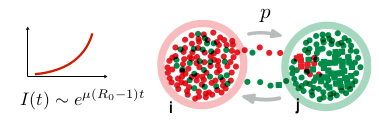
\includegraphics[width=0.7\textwidth]{../lessons/image/15/image01.png}
\caption{\label{fig:14_01} Dynamics of spatial spread: p is the traveling probability $i \to j$, and $I(t)$ is the prevalence in patch $j$ at time $t$.}
\end{figure}

Consequently, the probability that the \textit{first infectious} individual arrives at time $t_{\text{seeding}} = t = n\Delta t$ in city $j$ is then given by:
\begin{equation}
    P(t_{\text{seeding}}= n\Delta t ) = [1-(1-p)^{I(n\Delta t)}] \times  \prod_{i=1}^{n-1} (1-p)^{I(i \Delta t)}
\end{equation}
which expresses the fact that at least one successful “jump” from $i$ to $j$ of an infectious individual occurs at time $n \Delta t$, and none at previous times. In order to obtain the probability density of the arrival time in city $i$, we first note that in real world systems the number of travelers is usually small with respect to the total population of a city: $p = w\Delta t/N \ll 1$. In this limit for $p \to 0$, we can rewrite:
\begin{equation*}
    P(t_{\text{seeding}}=t) = pI(t)e^{-p\sum_{0 < i <n} I(i\Delta t)}
\end{equation*}
Using the standard approximation of $\Delta t \sum_{0 < i <n} I(i\Delta t) \to \int_0^t I(\tau)d\tau$:
\begin{equation}
     P(t_{\text{seeding}}=t) = p I(t) e^{-p\int_0^t I(\tau)d\tau}
\end{equation}
Defining now $a = \mu (R_0 - 1)$ and knowing that $I(t) = e^{at}$ at early stages, we can rewrite the probability as:
\begin{equation}
    P(t_{\text{seeding}}=t) = pe^{at}e^{-\frac{p}{a}e^{at}}
\end{equation}
That is a \textbf{Gumbel distribution}, whose expected value is:
\begin{equation}
    \expval{t_{\text{seeding}}} \simeq - \frac{1}{a} log\left(\frac{p}{a}\right)
\end{equation}
This is the expected time needed for the infection, starting in $i$, to end up in $j$ for a 2 patches model.
Let us consider now the generalization to a \textbf{chain} of identical patches (see fig \ref{fig:14_02}), denoting the population as $N$ and the traveling weight among patches $p$.

\begin{figure}[h!]
\centering
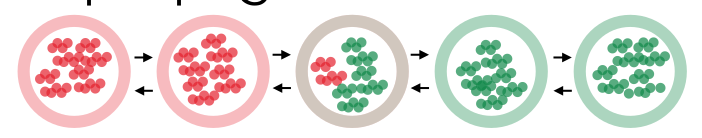
\includegraphics[width=0.7\textwidth]{../lessons/image/15/image02.png}
\caption{\label{fig:14_02} Dynamics of spatial spread: p is the traveling probability among patches, that are now more than two.}
\end{figure}

Now it occurs that there is \textbf{correlation} among patches, since the time at which the patch $i$ is infected does depend on the previous one, that in turn depends on the one before and so forth. Infected people that travel between patches are actually important only at the starting of each infection process for every patch, but later these can be neglected since their contribution is small compared to the normal spreading dynamics. We can define as $\Delta_i$ the interval that interoccurs between two consecutive seedings, obviously related to different patches:
\begin{equation}
    \expval{t_{\text{seeding}, i}} - \expval{t_{\text{seeding}, i - 1}} = \Delta_i, \qquad \expval{t_{\text{seeding}, n}} = \sum_{i=1}^n \Delta_i
\end{equation}
Consequently $\Delta_i$ are correlated and not identically distributed: incidence dynamics in city $i$ is mainly given by two contributions. The first is a term related the introduction of the infection from $i-1$-th patch (travelling rate, infected individual travelling...), while the second one is given by the infection transmission dynamics within patch $i$ itself. Every patch is therefore correlated to the previous ones. However, the simplest approximation one can think of is:
\begin{equation*}
    \expval{\Delta} = \expval{t_{\text{seeding}, 1}}
\end{equation*}
which can be shown to not work so bad\footnote{Gautreau et al JTB 2008.}.

It is straightforward to introduce a \textbf{metric} that describes how nodes are close to each other. It is function of connection “weights” (see Fig. \ref{fig:14_03}) that are in turn given by the number of travellers, of flights and connections are present between a pair of nodes. In this way we are able to introduce an \textbf{effective distance}\footnote{Brockmann, Helbing, Science 2013.}  $- \ln(p_{ij})$  between nodes $i$ and $j$: despite the geographical distance is way larger, it follows that New York and London are actually closer than New York and any other rural place in the US Midwest using this metric.

\begin{figure}[h!]
\centering
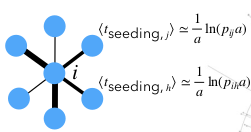
\includegraphics[width=0.3\textwidth]{../lessons/image/15/image03.png}
\caption{\label{fig:14_03} Effective distance between node $i$ and other nodes connected to it. The larger the edge, the stronger the connection weight.}
\end{figure}

So, the existence of \textbf{pathways}\footnote{Colizza, Barrat, Barthelemy et Vespignani, PNAS (2006).}, through which it is more likely that the spread of a disease can occur, comes in helpful when we are requested to make risk assessment analysis for some regions.
Indeed, it allows us to better \textbf{predict} the possible path through which the evolution of a spreading might occur. We now introduce the \textit{overlap function} $\Theta(t) \in [0,1]$ that describes the similarity between 2 outbreak realizations among different numerical simulations: the closer to 1, the more similar they are. Obviously, the \textbf{higher} the \textbf{overlap}, the \textbf{higher} the \textbf{predictability}.

\begin{figure}[h!]
\centering
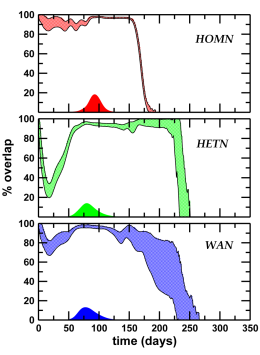
\includegraphics[width=0.35\textwidth]{../lessons/image/15/image04.png}
\caption{\label{fig:14_04}\\ \textbf{Top:} numerical simulations with no degree fluctuations and no weight fluctuations. \\ \textbf{Middle:} numerical simulations with only degree fluctuations and no weight fluctuations. \\ \textbf{Bottom:} numerical simulations with both degree fluctuations and weight fluctuations.}
\end{figure}

As one can clearly understand from Fig. \ref{fig:14_04}, introducing the \textbf{degree heterogeneity} decreases the predictability: in this way we are including hubs in our model. On the other hand, if we consider also \textbf{pathways} hence bringing in \textbf{weight fluctuations} numerical simulations are more likely to return similar outputs (the predictability is increased).


One of the most important questions when dealing with epidemics and mobility is whether introducing \textbf{travel bans} would allow us to gain some time wrt the spreading of the disease. In other words we want to see if a restriction of traffic would be \textbf{effective} in either containing or delaying the propagation\footnote{Gautreau et al JTB 2008; Hollingsworth et al Nature Med 2006; Scalia Tomba et al Math Biosci 2008.}.
We therefore \textit{rescale} the travelling probability by a factor of $\omega$:
\begin{equation}
    \expval{t_{\text{seeding}, T.R.}} \simeq  - \frac{1}{a} \ln( \frac{p \omega}{a})
\end{equation}
We can now compute how much time we “gain” when we introduce some traffic restrictions:
\begin{equation}
    \expval{t_{\text{seeding}, T.R.}} - \expval{t_{\text{seeding}}} \ \simeq \  - \frac{1}{a} \ln( \frac{p \omega }{a}) + \frac{1}{a} \ln(\frac{p}{a}) = - \frac{1}{a} \ln(\omega)
\end{equation}
where $ 0 < \omega \leqslant 1$. This result is indeed really important: to have a \textbf{consistent delay} in the propagation, we must \textbf{cut} the \textbf{flights} about \textbf{order of magnitudes}, with all possible consequent social and economical implications since the dependence is logarithmic. Therefore, the moral is that it is way \textit{better to help the metapopulation where the epidemic started}, rather than cutting flights, being it quite useless.
This would mean to try to decrease the slope of the exponential growth in the patch where the disease originated. For instance, during $H1N1$ pandemic in 2009, traffic volume from Mexico to Europe decreased by a factor of $40\%$, and the only gain in delay was really poor (order of days). Indeed, the same result is obtained thanks to numerical simulations with a global spreading model for influenza and it turn out that the delay is negligible.


We want now to briefly discuss how these arguments can be applied to \textbf{epidemic assessment}, in particular wrt \textbf{COVID-19} situation\footnote{\url{https://www.nytimes.com/interactive/2020/03/22/world/coronavirus-spread.html}\label{imp_college_ref}.}. One of the first early warnings emanated by the Wuhan Municipal Health Committee was the following: \emph{“urgent notice on the treatment of pneumonia of unknown cause”}. This was actually picked up by ProMED-mail, which is an independent program for emerging diseases, that raised an alert to the situation in Wuhan at the beginning of January. Later, some cases of pneumonia were discovered far from the epicentre among travellers, namely 2 in Thailand and 1 in Japan: compared to the 40 \textit{local} cases and to the traffic volume (i.e. $p$ to travel) it was really out of scale: local cases should have been many more. This argument was actually developed by the Imperial College, stating that\footnote{\url{https://www.imperial.ac.uk/mrc-global-infectious-disease-analysis/covid-19/report-1-case-estimates-of-covid-19/} \label{footnote:imp_college_ref}} this new pneumonia had already started spreading worldwide and provided an estimate for the number of cases. We want now to follow the argument developed by the just mentioned report. Clearly, the number of infected that travel is $I_{trav} = I_{Wuhan}\cdot p_{travel}$, where the probability that an infectious travels $p_{travel}$ is the product between the daily probability to travel $p_{daily}$ and the time to detect a case $T_d$:
\begin{equation}
    p_{travel} = p_{daily} T_d
\end{equation}
where $p_{daily}$ is the probability of travelling out of Wuhan, namely $p_{daily} = \frac{w}{N}$ and the time to detect a case $T_d$ is the sum of two terms: \textit{incubation period} and \textit{time to hospitalization} (first cases were detected only after hospitalization, i.e. when symptoms started to be severe).
Using real parameters, namely the passenger per day at Wuhan airport $w = 3301\ person/day$, the catchment population of the just mentioned airport $N\sim 10^6\ individuals$ and the incubation period $5-6\ days$ and time to hospitalization $4-5\ days$ we could infer that the estimated cases must have been around $1800\ (95\ \% C.I. : 427 - 4471)$ individuals. This is much more than the 40 cases officially detected. After that particular moment, with some delay, WHO raised an alert, too, and surveillance was heightened in foreign countries. Since mobility data among countries is actually more reliable, we can use them in order to infer the epidemiological situation in the seed country.


A tool used in \textbf{numerical simulations}, for the worldwide spread of epidemics, we may ever encounter is the website \url{http://www.gleamviz.org/}. GLEaM\footnote{\textbf{Gl}obal \textbf{E}pidemic \textbf{a}nd \textbf{M}obility Model.} is indeed a site that allows us to both visualize and simulate numerically the evolution of a pandemic using different data mobility and networks.



\subsection{SIR metapopulation model with memory}

Let us now discuss the \textbf{SIR metapopulation} model in a different regime: \textbf{commuting}\footnote{Sattenspiel, L. \& Dietz, K. Math. Biosci. 128, 71–91 (1995)} \footnote{Keeling, M. J. \& Rohani, P. Ecol. Lett. 5, 20–29 (2002)}, and not air travel any more. We therefore \textbf{drop} the \textbf{assumption} that the traveling rate is \textit{negligible} with respect to the epidemic time scale, i.e. $p_{ij} \ll \mu$. The interoccurrence time between two trips, from now on, will be of order of \textit{hours}: much less than the recovery rate.

In general, treating mathematically the interplay between mobility and transmission is very difficult. The problem can be solved by using \textbf{time scale separation}, that works as a sort of \textit{mean field approximation}. Hence, either the \textbf{epidemic unfolds faster than mobility}, that is the case of flu
($\mu \sim 10^{-1}\ days^{-1}$) and air traveling (rate $\sim 10^{-3} days^{-1}$ ) or alternatively \textbf{mobility is faster than the epidemics}, that is the case of commuting (usually we travel twice a day, its rate is $\sim 3 days^{-1}$) and flu ($\mu \sim 10^{-1} days^{-1}$). \textbf{Timescale} in \textit{commuting case} is mainly given by travel duration, whereas the \textbf{probability} $p$ instead determines the fraction of people commuting, i.e. the fraction of workers/students that daily travel vs pensioners that do not.

\begin{figure}[h!]
\centering
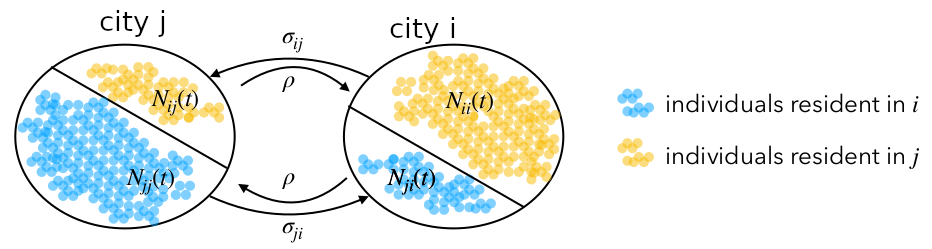
\includegraphics[width=1\textwidth]{../lessons/image/15/image05.png}
\caption{\label{fig:14_05} Graphical representation for the SIR metapopulation model with memory, this is actually more realistic since we usually back and forth in such trips home$\xleftrightarrow[]{}$workplace. We distinguish the population inside patches on their residence place. }
\end{figure}

We want now to take into account that, when \textbf{commuting}, we usually \textbf{return} to the place where we started. A typical trip in this case would be $i \xrightarrow{} j \xrightarrow[]{} i$. Nothing however prevents us to leave once again for $k$-th patch as soon as we are back to $i$, but this would not not commuting any more. The first modification we make is to divide every patch (here for simplicity we show only two in Fig. \ref{fig:14_05}) distinguishing on the individuals and whether they are resident in $i$ or $j$. In this way we can consider people that, despite they live in another patch $i$, travelled to patch $j$ with a certain \textbf{leaving rate} $\sigma_{ij}$ and will return home according to a \textbf{returning rate} $\rho^{-1} = \tau \approx 8h$.
that is independent of the destination. $N_{ij}(t)$ are the individuals resident in $i$ and traveling to $j$, while we approximate the \textbf{population} for a given patch $i$ as \textit{constant}:
\begin{equation}
    N_i = N_{ii}(t) + \sum_{j} N_{ij}(t)
    \label{eqn:popul_N}
\end{equation}
The latter is the expression that describes the number of people \textbf{resident} in patch $i$. In other words we are assuming no immigration and no births nor deaths. In this way we can keep track of from where and individual left.

We want now to consider the the change in time of people resident in $i$ and either staying in $i$ or leaving for $j$:
\begin{subequations}
\begin{align}
    \partial_t N_{ii}(t) &= - \sum_{j} \sigma_{ij} N_{ii}(t) + \rho \sum_{j} N_{ij} (t)\\
    \partial_t N_{ij}(t) &= \sigma_{ij} N_{ii}(t) - \rho N_{ij}(t)
\end{align}
\end{subequations}
The linear ordinary \textbf{differential equation} of order 1 to be solved can be rewritten, replacing $\sum_{j} N_{ij}(t)$ from \ref{eqn:popul_N} into $\partial_t N_{ii}(t)$, as:
\begin{equation}
    \partial_t N_{ii} (t) + (\rho + \sigma_i) N_{ii}(t) = N_i \rho
\end{equation}
The first solution is:
\begin{equation}
\begin{split}
    N_{ii}(t) &= e^{(\rho + \sigma_i)t}\left( C_ii + N_i \rho \int_0^t e^{(\rho + \sigma_i)s}ds \right)=\\
     &= \frac{N_i}{1+\sigma_i/\rho} + \left( N_{ii}(0) - \frac{N_i}{1+\sigma_i/\rho} \right) e^{-\rho(1+\sigma_i/\rho)t}
\end{split}
\end{equation}
While for the individuals resident in $i$ and travelling to $j$:
\begin{equation}
\begin{split}
    N_{ij}(t) &= \frac{\sigma_{ij}N_i/\rho}{1+\sigma_i/\rho} - \frac{\sigma_{ij}}{\sigma_i} \left( N_{ii}(0) - \frac{N_i}{1+\sigma_i/\rho} \right) e^{-\rho(1+\sigma_i/\rho)t} +\\
    &+ \left[ N_{ii}(0) - \frac{\sigma_{ij}N_i/\rho}{1+\sigma_i/\rho} -\frac{\sigma_{ij}}{\sigma_i} \left( N_{ii}(0) - \frac{N_i}{1+\sigma_i/\rho} \right)\right] e^{-\rho t}
\end{split}
\end{equation}
More important quantity to be defined is the \textbf{time of relaxation} to the equilibrium, which is defined as $\tau$ and dominated by:
\begin{equation}
    [\rho(1+\sigma_i/\rho)]^{-1} \sim \rho^{-1} = \tau \qquad \text{since } \rho \gg \sigma_i
\end{equation}
where the probability of leaving $i$ regardless the destination is $\sigma_i = \sum_{j} \sigma_{ij}$
Therefore, the \textbf{equilibrium solutions} one may find are:
\begin{equation}
    N_{ii} = \frac{N_i}{1+\sigma_i/\rho}, \qquad N_{ij} = \frac{\sigma_{ij}N_i/\rho}{1+\sigma_i/\rho}
\end{equation}
Since also in the \textbf{steady state} number of people that are \textit{resident} in $i$ is conserved, then we can compute the number of people $\textbf{present}$ in $i$ as:
\begin{equation}
    N_i^* = N_{ii} + \sum_{j}N_{ji} = \frac{N_i}{1+\sigma_i/\rho} + \sum_j \frac{N_j \sigma_{ji}/\rho}{1+\sigma_j/\rho}
    \label{eqn:N^*}
\end{equation}
The ratio actually $\sigma_i/\rho$ quantifies the proportion of time spent outside and in the residence population.


Let us discuss now some \textbf{limiting cases}:
\begin{itemize}
    \item $\sigma_i \to 0 \implies N_{ii}(t) \to N_i;\ N_{ij}(t) \to 0;\ N_i^*\to N_i$ in this case people rarely leave their residence, thus the non travelling individuals approach the population of residents;
    \item $\rho \to \infty \implies N_{ii}(t) \to N_i;\ N_{ij}(t) \to 0;\ N_i^*\to N_i$ people return home immediately thus the non travelling individuals approach the population of residents;
    \item $\rho \to 0 \implies N_{ii}(t) \to 0;\ N_{ij}(t) \to \frac{\sigma_{ij}}{\sigma_i}N_i;\ N_i^*\to \sum_j \frac{\sigma_{ji}}{\sigma_j} N_j$ here the case collapses to \textbf{migration} process: people never get back and the population of resident in $i$ is distributed among the neighbouring destinations $j$.
\end{itemize}

One should recall now that the time scale of commuting $\tau \approx 8\,\text{h}$, while the duration of an acute infection (i.e. flu) is way more: $\mu^{-1} \approx [1-3]\, \text{days}$. We could adopt, as said, a \textit{mean field} paradigm: we assume that the person can be partially in a place and partially in another one: on average it happens that he might be at the same time in different places\footnote{in terms of reality it is meaningless to state that fractions of person are present in different places, unless we are speaking about Voldemort and his Horcruxes. Aside jokes, Mean Field approximation allows us to attach a meaning to these fractions since we are considering them "on average".}. \textbf{Transmission dynamics} is therefore \textbf{slower than mobility}: we can assume that compartments occupation numbers are at the equilibrium with respect to mobility dynamics. Formally, the \textbf{occupation numbers} are:
\begin{equation}
    X_{ii}^{[m]} = \frac{X_i^{[m]}}{1+\sigma_i/\rho}, \quad X_{ij}^{[m]} = \frac{\sigma_{ij}X_i^{[m]}/\rho}{1+\sigma_i/\rho}, \quad X^{[m]} = S,I,R
\end{equation}
We want now to understand how many infected individuals a susceptible person resident in $i$ is exposed to, that is to say we want to compute the \textbf{force of infection} $\lambda$:
\begin{equation}
    \lambda = \beta \frac{I(t)}{N(t)}
\end{equation}
This parameter is present in the set of differential equations related to compartments numbers:
\begin{subequations}
\begin{align}
    \partial_t S &= -\beta \frac{I(t)}{N(t)} S(t)\\
    \partial_t I &= \beta \frac{I(t)}{N(t)} S(t) - \mu I (t) = \lambda S(t) - \mu I (t)\\
    \partial_t R &= \mu I(t)
\end{align}
\end{subequations}

Instead of explicitly modelling mobility, we now directly compute the effects of the other patches on the risk of infection, i.e. we break down the force of infection in its different contributions.
Having assumed we are at equilibrium, $S_i$ is distributed among patch $i$ and all possible destinations $j$ according to the set of proportions:
\begin{equation*}
    \qty{ \frac{1}{1+\sigma_i/\rho}, \dots , \frac{\sigma_{ij}/\rho}{1+\sigma_i/\rho}, \dots  }
\end{equation*}
whereas the \textbf{risk of infection} has the form:
\begin{equation}
    \lambda_i = \frac{\lambda_{ii}}{1+\sigma_i/\rho} + \sum_{j} \frac{\lambda_{ij}\sigma_{ij}/\rho}{1+\sigma_i/\rho}
\end{equation}
where the first contribution is the contribution of people that stay at home, and the second is the contribution of people infected that visit patch $i$ from any other patch $j$.
In the formula above we have that $\lambda_{ii}$ is the force of infection that a person resident $i$ experiences from infected people that are in $i$, formally:
\begin{equation}
    \lambda_{ii} = \frac{\beta_i}{N_i^*} \qty[ I_{ii} + \sum_j I_{ji} ] = \frac{\beta_i}{N_i^*} \qty[ \frac{I_i}{1+\sigma_i/\rho} + \sum_j \frac{I_j \sigma_{ji}/\rho}{1+\sigma_j/\rho} ]
\end{equation}
Whereas $\lambda_{ij}$ is the contribution of a susceptible resident in $i$ that is travelling to any other patch $j$ and there is exposed to infected people:
\begin{equation}
    \lambda_{ij} = \frac{\beta_j}{N_j^*} \qty[ I_{jj} + \sum_l I_{lj} ] = \frac{\beta_j}{N_j^*} \qty[ \frac{I_j}{1+\sigma_j/\rho} + \sum_l \frac{I_l \sigma_{lj}/\rho}{1+\sigma_{l}/\rho} ]
    \label{eqn:lambda_ij}
\end{equation}
Note as some of the terms are similar to the steady state ones in equation \ref{eqn:N^*}. These last expressions are actually useful in \textbf{numerical simulations}, and they allow us to understand the relative role of mobility and infection parameters on the epidemic dynamics in order to speed up the simulations, too. One should actually remember that both \textit{infections} and \textit{travels} are \textbf{stochastic processes}, and last results hold only when mobility is faster than the epidemics time scale.


\end{document}
